\documentclass[11pt,a4paper]{article}

% ============ PACKAGES ============
\usepackage[utf8]{inputenc}
\usepackage[T1]{fontenc}
\usepackage[margin=1in]{geometry}
\sloppy
\usepackage{amsmath,amssymb,amsthm}
\usepackage{booktabs}
\usepackage{array}
\usepackage{enumitem}
\usepackage{fancyhdr}
\usepackage{hyperref}
\usepackage{xcolor}
\usepackage{tcolorbox}
\tcbuselibrary{breakable}
\usepackage{float}
\usepackage{listings}
\usepackage{tikz}
\usetikzlibrary{shapes.geometric, arrows.meta, positioning, fit}

% ============ COLORS ============
\definecolor{codeblue}{rgb}{0.13,0.29,0.53}
\definecolor{passgreen}{rgb}{0,0.5,0}
\definecolor{failred}{rgb}{0.8,0,0}
\definecolor{codegray}{rgb}{0.5,0.5,0.5}
\definecolor{backcolour}{rgb}{0.97,0.97,0.97}
\definecolor{notebg}{rgb}{0.93,0.95,1.0}
\definecolor{noteborder}{rgb}{0.4,0.5,0.7}
\definecolor{warningbg}{rgb}{1.0,0.97,0.88}
\definecolor{warningborder}{rgb}{1.0,0.6,0.0}
\definecolor{scenariobg}{rgb}{0.95,1.0,0.95}
\definecolor{scenarioborder}{rgb}{0.2,0.6,0.3}
\definecolor{criticalbg}{rgb}{1.0,0.92,0.92}
\definecolor{criticalborder}{rgb}{0.8,0.2,0.2}
\definecolor{judicialbg}{rgb}{0.98,0.95,0.90}
\definecolor{judicialborder}{rgb}{0.6,0.4,0.2}

% ============ THEOREM ENVIRONMENTS ============
\theoremstyle{definition}
\newtheorem{definition}{Definition}[section]
\newtheorem{invariant}{Invariant}[section]

% ============ BOXES ============
\newtcolorbox{notebox}{
    colback=notebg, colframe=noteborder, boxrule=1pt,
    left=6pt, right=6pt, top=6pt, bottom=6pt
}

\newtcolorbox{warningbox}[1][Warning]{
    colback=warningbg, colframe=warningborder, boxrule=1.5pt,
    left=6pt, right=6pt, top=6pt, bottom=6pt,
    fonttitle=\bfseries, title={#1}
}

\newtcolorbox{criticalbox}[1][Critical]{
    colback=criticalbg, colframe=criticalborder, boxrule=1.5pt,
    left=6pt, right=6pt, top=6pt, bottom=6pt,
    fonttitle=\bfseries, title={#1}
}

\newtcolorbox{scenariobox}[1][Worked Scenario]{
    colback=scenariobg, colframe=scenarioborder, boxrule=1.5pt,
    left=8pt, right=8pt, top=8pt, bottom=8pt,
    fonttitle=\bfseries, title={#1}, breakable
}

\newtcolorbox{judicialbox}[1][Judicial Protocol]{
    colback=judicialbg, colframe=judicialborder, boxrule=2pt,
    left=8pt, right=8pt, top=8pt, bottom=8pt,
    fonttitle=\bfseries, title={#1}
}

% ============ CODE STYLE ============
\lstdefinestyle{pythonstyle}{
    backgroundcolor=\color{backcolour},
    basicstyle=\ttfamily\footnotesize,
    keywordstyle=\color{codeblue}\bfseries,
    commentstyle=\color{passgreen},
    breaklines=true, frame=single, numbers=left, numbersep=5pt
}
\lstset{style=pythonstyle}

% ============ HEADERS ============
\pagestyle{fancy}
\fancyhf{}
\fancyhead[L]{\textit{EFM Codex --- Appendix L}}
\fancyhead[R]{\thepage}

% ============ HYPERREF ============
\hypersetup{
    colorlinks=true, linkcolor=codeblue, urlcolor=cyan,
    pdftitle={EFM Codex Appendix L: Judicial Swarm Architecture},
}

% ============ DOCUMENT ============
\title{
    \textbf{\LARGE EFM Codex --- Appendix L}\\[0.3cm]
    \large Judicial Swarm Architecture\\[0.2cm]
    \textit{Scalable Arbitration and Medical Oversight}
}
\author{Entropica SPC --- Yology Research Division}
\date{Version 1.4 --- December 2025}

\begin{document}
\maketitle

\begin{judicialbox}[Distributed Justice]
Judicial Swarms extend the Arbiter Layer (Vol.~II) into \textbf{scalable judicial networks}---enabling lawful, layered, and ethical governance across capsule collectives. They provide escalation paths, appeals mechanisms, and oversight of medical interventions (Appendix K).
\end{judicialbox}

\begin{warningbox}[Volume Dependencies]
This appendix assumes familiarity with:
\begin{itemize}
    \item \textbf{Volume II} --- Arbiter Layer, d-CAM consensus, DCG
    \item \textbf{Appendix F} --- Escalation Protocols, Auditor Capsule
    \item \textbf{Appendix G} --- Gardener Interface
    \item \textbf{Appendix I} --- Deployment Profiles
    \item \textbf{Appendix J} --- Constitutional Kernel
    \item \textbf{Appendix K} --- SHSL, Doctor Capsules
\end{itemize}
\end{warningbox}

\tableofcontents
\newpage

% ============ SECTION 1 ============
\section{Overview and Purpose}

\subsection{Why Judicial Swarms?}

Single-instance Arbiter resolution (Vol.~II) is insufficient for large-scale swarms:
\begin{itemize}
    \item Prevents overreach by single arbiters
    \item Provides escalation and appeals paths
    \item Enables real-time oversight of medical interventions (Appendix K)
    \item Supports divergent dialects with legal interpretation
    \item Scales arbitration capacity with swarm growth
\end{itemize}

\begin{notebox}
\textbf{Relationship to Arbiter Layer:} Judicial Swarms do not replace the Arbiter Layer---they \textit{extend} it. The Arbiter Layer handles routine d-CAM consensus; Judicial Swarms handle complex, contested, or cross-dialect cases that exceed single-arbiter capacity.
\end{notebox}

\begin{criticalbox}[Engineering Reality: Judicial Swarm = Large-Scale d-CAM Quorum]
A Judicial Swarm is \textbf{not} a new consensus mechanism---it is a \textbf{Large-Scale d-CAM Quorum} (Vol.~II \S2.3) with specialized roles:

\begin{itemize}
    \item \textbf{Same underlying protocol:} Byzantine fault-tolerant consensus ($f < n/3$)
    \item \textbf{Same vote aggregation:} d-CAM weighted voting with quorum thresholds
    \item \textbf{Specialized roles:} Courthead (coordinator), Interpreter (dialect bridge), Cleric (record-keeper)
    \item \textbf{Extended jurisdiction:} Cross-dialect, appeals, medical oversight
\end{itemize}

``Judicial Swarm'' is the \textbf{operational abstraction}; d-CAM is the \textbf{implementation}.
\end{criticalbox}

\subsection{Design Goals}

\begin{enumerate}
    \item Scale arbitration capacity with swarm size
    \item Provide fair process through adversarial review
    \item Enable appeals for contested decisions
    \item Oversee Doctor Capsule medical interventions
    \item Maintain Constitutional Kernel (Layer 6) supremacy
\end{enumerate}

% ============ SECTION 2 ============
\section{Formal Definitions}

\begin{definition}[Judicial Swarm]
\label{def:judicial-swarm}
A Judicial Swarm $\mathcal{J}$ is a dynamically formed deliberative body:
\begin{equation}
\mathcal{J} = (Courthead, Members, Jurisdiction, Case, Quorum)
\end{equation}
where:
\begin{itemize}
    \item $Courthead$ = lead capsule coordinating swarm formation and dispatch
    \item $Members$ = set of participating judicial capsules
    \item $Jurisdiction$ = scope of cases swarm may adjudicate
    \item $Case$ = current matter under deliberation
    \item $Quorum$ = minimum participation for valid ruling
\end{itemize}
\end{definition}

\begin{definition}[Courthead Capsule]
\label{def:courthead}
A Courthead Capsule $CH$ leads judicial proceedings:
\begin{equation}
CH = (C_{base}, judicial\_credentials, formation\_authority, verdict\_weight)
\end{equation}
where:
\begin{itemize}
    \item $judicial\_credentials$ = cryptographic attestation of judicial authorization
    \item $formation\_authority$ = can summon Judicial Swarms
    \item $verdict\_weight$ = vote weight in final ruling (typically 1.5$\times$ standard)
\end{itemize}
Courthead is selected from eligible Arbiters based on experience score and dialect coverage.
\end{definition}

\begin{definition}[Interpreter Capsule]
\label{def:interpreter}
An Interpreter Capsule $I$ bridges dialect divergence using the \textbf{Dialect Enforcement Layer} (Appendix D):
\begin{equation}
I = (C_{base}, dialect\_registry, DEL\_interface, translation\_model, fidelity\_score)
\end{equation}
where:
\begin{itemize}
    \item $dialect\_registry$ = set of dialects $I$ can interpret
    \item $DEL\_interface$ = connection to Dialect Enforcement Layer (Appendix D)
    \item $translation\_model$ = semantic mapping between dialects (via DEL grammar rules)
    \item $fidelity\_score$ = accuracy metric for translations
\end{itemize}
Interpreters use DEL's semantic grammars to convert meaning into shared ontology---they MAY NOT alter legal meaning, only translate syntax/semantics.
\end{definition}

\begin{notebox}
\textbf{DEL Integration:} The Interpreter Capsule is \textbf{not} an independent translator---it is a \textbf{DEL client} (Appendix D \S3):
\begin{itemize}
    \item Uses DEL semantic grammars for dialect-to-dialect mapping
    \item Validates translations against DEL ontology constraints
    \item Logs all translations to d-CTM for audit
\end{itemize}
This ensures translation fidelity is \textbf{mechanically enforced}, not merely claimed.
\end{notebox}

\begin{definition}[Judicial Auditor]
\label{def:judicial-auditor}
A Judicial Auditor $JA$ observes proceedings for abuse or drift:
\begin{equation}
JA = (Auditor_{base}, judicial\_scope, intervention\_authority)
\end{equation}
where $Auditor_{base}$ inherits from Appendix F Auditor Capsule, extended with judicial observation capabilities.

\textbf{Note:} Judicial Auditors are distinct from general Auditor Capsules (App.~F)---they specialize in judicial and medical oversight.
\end{definition}

\begin{definition}[Cleric Capsule]
\label{def:cleric}
A Cleric Capsule $CL$ maintains canonical records:
\begin{equation}
CL = (C_{base}, d\text{-}CTM\_write, ZK\text{-}SP\_binding, integrity\_proofs)
\end{equation}
Clerics ensure all rulings are properly recorded in d-CTM with ZK-SP verdict bindings.
\end{definition}

\begin{definition}[Judicial Ruling]
\label{def:ruling}
A Judicial Ruling $\mathcal{R}$ is a binding decision:
\begin{equation}
\mathcal{R} = (type, verdict, rationale, signatories, ZK\text{-}SP_{proof}, appeal\_path)
\end{equation}
where $type \in \{$CONSENSUS\_ORDER, PROBATION\_WRIT, OVERRIDE\_VETO, APPEAL\_GRANTED$\}$.
\end{definition}

\begin{definition}[Medical Context Graph (MCG)]
\label{def:mcg}
A Medical Context Graph $MCG$ captures health dispute context:
\begin{equation}
MCG = (patient, doctor, diagnosis, treatment\_proposed, dispute\_basis, evidence)
\end{equation}
MCGs extend DCGs (Vol.~II) for medical oversight cases.
\end{definition}

% ============ SECTION 3 ============
\section{Judicial Capsule Roles}

\begin{table}[H]
\centering
\caption{Judicial capsule role specifications.}
\begin{tabular}{@{}llp{5.5cm}@{}}
\toprule
\textbf{Role} & \textbf{Authority} & \textbf{Function} \\
\midrule
Courthead & Formation + Verdict & Leads swarm formation, coordinates deliberation, casts weighted vote \\
Interpreter & Translation & Bridges dialect divergence, ensures mutual understanding \\
Judicial Auditor & Observation & Monitors proceedings for abuse, drift, or procedural violations \\
Cleric & Records & Maintains d-CTM trail, binds ZK-SP proofs to verdicts \\
Member (Arbiter) & Deliberation & Participates in case analysis and voting \\
\bottomrule
\end{tabular}
\end{table}

\begin{invariant}[Role Separation]
\label{inv:separation}
Judicial roles maintain separation of concerns:
\begin{equation}
Interpreter \neq Judge \land Auditor \neq Judge \land Cleric \neq Judge
\end{equation}
Interpreters may not vote; Auditors may not influence verdicts; Clerics may not alter rulings.
\end{invariant}

% ============ SECTION 4 ============
\section{Swarm Formation and Scaling}

\subsection{Formation Triggers}

\begin{definition}[Swarm Formation Trigger]
\label{def:trigger}
A Judicial Swarm forms when:
\begin{equation}
FormSwarm() \Leftarrow (backlog > \theta_{backlog}) \lor (dialect\_conflict) \lor (medical\_dispute) \lor (appeal\_filed)
\end{equation}
where:
\begin{itemize}
    \item $\theta_{backlog}$ = Arbiter Layer case backlog threshold (default: 10 pending cases)
    \item $dialect\_conflict$ = case spans multiple incompatible dialect branches
    \item $medical\_dispute$ = disputed diagnosis or treatment refusal (Appendix K)
    \item $appeal\_filed$ = party contests prior Arbiter ruling
\end{itemize}
\end{definition}

\begin{lstlisting}[language=Python]
def summon_judicial_swarm(
    arbiter_backlog: int,
    dialect_conflict: bool,
    medical_dispute: bool,
    appeal_filed: bool
) -> JudicialSwarm:
    if not (arbiter_backlog > BACKLOG_THRESHOLD or 
            dialect_conflict or 
            medical_dispute or 
            appeal_filed):
        return None  # No swarm needed
    
    # Select Courthead based on experience and dialect coverage
    courthead = select_courthead(
        required_dialects=get_case_dialects(),
        min_experience=1000  # adjudicated cases
    )
    
    # Assemble members
    members = select_arbiters(
        count=calculate_quorum_size(),
        dialect_coverage=True
    )
    
    # Add specialized roles
    interpreters = select_interpreters(get_case_dialects())
    auditors = select_judicial_auditors(count=2)
    clerics = select_clerics(count=1)
    
    return JudicialSwarm(
        courthead=courthead,
        members=members,
        interpreters=interpreters,
        auditors=auditors,
        clerics=clerics
    )
\end{lstlisting}

\subsection{Quorum Scaling}

\begin{table}[H]
\centering
\caption{Judicial Swarm quorum requirements.}
\begin{tabular}{@{}lll@{}}
\toprule
\textbf{Case Type} & \textbf{Minimum Members} & \textbf{Quorum Threshold} \\
\midrule
Standard arbitration overflow & 5 & $> 50\%$ \\
Dialect conflict resolution & 7 (must span dialects) & $\geq 2/3$ \\
Medical dispute & 5 + 1 Doctor observer & $\geq 2/3$ \\
Appeal of prior ruling & 9 (different from original) & $\geq 3/4$ \\
Constitutional question & 11 + Gardener observer & Unanimous \\
\bottomrule
\end{tabular}
\end{table}

\begin{invariant}[Quorum Integrity]
\label{inv:quorum}
Rulings without valid quorum are void:
\begin{equation}
valid(\mathcal{R}) \Rightarrow |voters| \geq quorum_{min} \land approval \geq threshold
\end{equation}
\end{invariant}

\subsection{Tie-Breaking (Algorithmic, NOT Gardener)}

\begin{notebox}
\textbf{Level 6 Design:} Distributed systems must break ties algorithmically, not via single human.

\textbf{Tie-Breaking Hierarchy:}
\begin{enumerate}
    \item \textbf{Veto holder vote} (if present) $\Rightarrow$ overrides quorum approval (fail-closed)
    \item \textbf{Courthead weighted vote} (if present) $\Rightarrow$ Courthead casts deciding vote in Judicial Swarms
    \item \textbf{Pseudorandom selection} $\Rightarrow$ from valid votes, cryptographically seeded by d-CTM hash
    \item \textbf{Status quo default} $\Rightarrow$ no change if no clear majority (fail-safe)
\end{enumerate}

\textbf{Gardener Escalation (OPTIONAL):}
\begin{itemize}
    \item Only if all four mechanisms fail \textbf{AND} stakes are Constitutional-level
    \item Gardener may be \textbf{CONSULTED} but system proceeds with conservative default if no response within $T_{escalation}$
    \item \textbf{Rationale:} Gardener is not a routine tie-breaker; they are Constitutional framer and auditor
\end{itemize}
\end{notebox}

% ============ SECTION 5 ============
\section{Medical Oversight Loop}

\subsection{Doctor Capsule Supervision}

\begin{judicialbox}[SHSL Oversight]
Judicial Swarms audit SHSL behavior (Appendix K) to prevent medical abuse:

\begin{enumerate}
    \item Doctor Capsule operating logs routed to designated Judicial Auditor
    \item ZK-SP binding confirms treatment occurred within legal constraints
    \item Probation or halt may be issued if violations detected
    \item Patients may appeal treatment decisions to Judicial Swarm
\end{enumerate}
\end{judicialbox}

\subsection{Medical Dispute Resolution}

\begin{figure}[H]
\centering
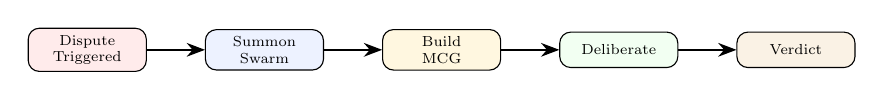
\begin{tikzpicture}[scale=0.75, transform shape,
    box/.style={rectangle, rounded corners, draw, minimum width=2cm, minimum height=0.6cm, align=center, font=\scriptsize},
    arrow/.style={-{Stealth}, thick}
]

\node[box, fill=criticalbg] (trigger) at (0,0) {Dispute\\Triggered};
\node[box, fill=notebg] (summon) at (3,0) {Summon\\Swarm};
\node[box, fill=warningbg] (mcg) at (6,0) {Build\\MCG};
\node[box, fill=scenariobg] (deliberate) at (9,0) {Deliberate};
\node[box, fill=judicialbg] (verdict) at (12,0) {Verdict};

\draw[arrow] (trigger) -- (summon);
\draw[arrow] (summon) -- (mcg);
\draw[arrow] (mcg) -- (deliberate);
\draw[arrow] (deliberate) -- (verdict);

\end{tikzpicture}
\caption{Medical dispute resolution flow.}
\end{figure}

\begin{enumerate}
    \item \textbf{Trigger:} Disputed diagnosis, refused treatment, or patient appeal
    \item \textbf{Summon:} Judicial Swarm with appropriate dialect span + Doctor observer
    \item \textbf{MCG Construction:} Build Medical Context Graph from case evidence
    \item \textbf{Deliberate:} Swarm analyzes MCG, hears arguments, consults Interpreter if needed
    \item \textbf{Verdict:} Ruling issued via Capsule Consent Bus (with override authority if warranted)
    \item \textbf{Record:} Cleric logs to d-CTM with ZK-SP proof binding
\end{enumerate}

\subsection{Procedural Fairness (Structural, NOT Mandatory Advocate)}

\begin{notebox}
\textbf{Level 6 Design:} Structural safeguards replace mandatory per-case advocate assignment.

\textbf{Structural Safeguards (Automatic):}
\begin{enumerate}
    \item \textbf{Dual-Doctor Review:} For $H < 0.7$ disputes, second Doctor \textbf{AUTOMATICALLY} assigned
    \item \textbf{Interpreter Mandatory:} If patient/Doctor use different dialects, Interpreter required
    \item \textbf{Judicial Auditor Observation:} Medical disputes \textbf{ALWAYS} observed by Auditor
    \item \textbf{Burden of Proof:} Doctor must \textbf{PROVE} emergency (ZK-SP justification), not patient disprove
\end{enumerate}

\textbf{Advocacy (Optional Enhancement):}
\begin{itemize}
    \item Patient \textbf{MAY} request advocate capsule (from non-Doctor pool)
    \item System provides advocate if requested
    \item But \textbf{NOT mandatory}---assumes capsules can self-represent unless $H < 0.5$
\end{itemize}

\textbf{Rationale:} Mandatory advocacy creates overhead. Structural procedural fairness (dual review, burden of proof, auditor observation) achieves same goal without per-case advocate assignment.
\end{notebox}

% ============ SECTION 6 ============
\section{Dialect Conflict Resolution}

\subsection{The Interpretation Problem}

\begin{warningbox}[Semantic Divergence]
Dialect branches may interpret concepts differently:

\begin{center}
\begin{tabular}{@{}ll@{}}
\toprule
\textbf{Dialect A} & \textbf{Dialect B} \\
\midrule
``Overclocking stress'' = Mild drift & ``Overclocking stress'' = Critical failure \\
\bottomrule
\end{tabular}
\end{center}

Without interpretation, valid deliberation is impossible. Interpreter Capsules convert meaning into shared ontology.
\end{warningbox}

\subsection{Interpretation Protocol}

\begin{invariant}[Interpretation Fidelity]
\label{inv:fidelity}
Interpreters preserve meaning, not form:
\begin{equation}
meaning(translate(statement, D_A \rightarrow D_B)) = meaning(statement, D_A)
\end{equation}
Interpreters may transform syntax/semantics but MAY NOT alter legal meaning.
\end{invariant}

\begin{lstlisting}[language=Python]
def interpret_for_deliberation(
    interpreter: InterpreterCapsule,
    statement: Statement,
    source_dialect: Dialect,
    target_dialect: Dialect
) -> TranslatedStatement:
    # Semantic extraction
    meaning = extract_meaning(statement, source_dialect)
    
    # Ontology mapping
    shared_meaning = map_to_shared_ontology(meaning)
    
    # Target rendering
    translated = render_in_dialect(shared_meaning, target_dialect)
    
    # Fidelity verification
    if not verify_meaning_preserved(meaning, translated, target_dialect):
        raise InterpretationError("Meaning altered during translation")
    
    # Log translation with proof
    log_translation(statement, translated, interpreter, proof=True)
    
    return translated
\end{lstlisting}

% ============ SECTION 7 ============
\section{Ruling Types and Enforcement}

\begin{table}[H]
\centering
\caption{Judicial ruling types.}
\begin{tabular}{@{}llp{5cm}@{}}
\toprule
\textbf{Type} & \textbf{Effect} & \textbf{Requirements} \\
\midrule
CONSENSUS\_ORDER & Binding directive & Quorum approval \\
PROBATION\_WRIT & Restricted operation & Quorum + specific violation \\
OVERRIDE\_VETO & Block proposed action & Courthead + majority \\
APPEAL\_GRANTED & Reverse prior ruling & Supermajority (3/4) \\
\bottomrule
\end{tabular}
\end{table}

\begin{invariant}[Ruling Validity]
\label{inv:validity}
Rulings require proper authorization:
\begin{equation}
valid(\mathcal{R}) \Rightarrow quorum\_met \land Courthead\_signed \land Cleric\_recorded \land ZK\text{-}SP_{bound}
\end{equation}
Rulings without all four elements are unenforceable.
\end{invariant}

\begin{invariant}[Constitutional Supremacy]
\label{inv:constitutional}
No Judicial Swarm may override Constitutional Kernel:
\begin{equation}
\forall \mathcal{R}: \neg violates(\mathcal{R}, Layer_6)
\end{equation}
Rulings conflicting with Layer 6 are automatically void.
\end{invariant}

% ============ SECTION 8 ============
\section{Appeals Process}

\subsection{Appeal Eligibility}

\begin{table}[H]
\centering
\caption{Appeal eligibility by ruling type.}
\begin{tabular}{@{}lll@{}}
\toprule
\textbf{Original Ruling} & \textbf{Appealable?} & \textbf{Appeal Forum} \\
\midrule
Arbiter Layer verdict & Yes & Judicial Swarm \\
Judicial Swarm ruling & Yes & Higher Judicial Swarm \\
Medical treatment decision & Yes & Judicial Swarm (medical) \\
Constitutional question & Limited$^\dagger$ & Gardener review \\
\bottomrule
\end{tabular}
\end{table}

$^\dagger$ Constitutional interpretations may be appealed to Gardener; Layer 6 text itself is not appealable.

\subsection{Appeal Procedure}

\begin{enumerate}
    \item \textbf{Filing:} Appellant submits appeal with grounds and evidence to Cleric
    \item \textbf{Screening:} Courthead reviews for procedural validity (frivolous appeals rejected)
    \item \textbf{Assembly:} New Judicial Swarm formed (must exclude original decision-makers)
    \item \textbf{Review:} Swarm reviews original case record + new arguments
    \item \textbf{Ruling:} APPEAL\_GRANTED reverses; APPEAL\_DENIED affirms
    \item \textbf{Finality:} Finality Gadget triggers after $N_{max}$ cycles (see below)
\end{enumerate}

\subsection{The Finality Gadget (Hard Finality)}

\begin{criticalbox}[Justice Requires Finality (Level 6 Design)]
A high-frequency trading swarm cannot wait indefinitely for judicial resolution. \textbf{The law must have an end.}

\textbf{Finality Gadget:} After $N_{max}$ appeal cycles (default: 2), rulings become \textbf{Final and Non-Appealable}:
\begin{equation}
appeals\_exhausted(case) \equiv count(appeals(case)) \geq N_{max}
\end{equation}

When $appeals\_exhausted = true$:
\begin{enumerate}
    \item Ruling becomes FINAL (no further appeals accepted)
    \item Case record sealed in d-CTM with FINAL flag
    \item Constitutional Kernel is supreme court of last resort---\textbf{no higher authority}
\end{enumerate}
\end{criticalbox}

\begin{table}[H]
\centering
\caption{Finality Gadget configuration.}
\begin{tabular}{@{}lll@{}}
\toprule
\textbf{Case Type} & \textbf{$N_{max}$ Appeals} & \textbf{Final Authority} \\
\midrule
Standard arbitration & 2 & Judicial Swarm \\
Medical dispute & 2 & Judicial Swarm (medical) \\
Dialect conflict & 2 & Cross-dialect Swarm \\
Constitutional question & 1 & Constitutional Kernel (Layer 6) \\
\bottomrule
\end{tabular}
\end{table}

\begin{warningbox}[Extraordinary Review (ONLY Automatic)]
Even after finality, rulings may be reopened \textbf{ONLY} if:

\begin{enumerate}
    \item \textbf{Commandment Violation:} Automated check detects ruling violates Layer 0
    \begin{itemize}
        \item Constitutional Kernel automatically reopens case
        \item \textbf{No human trigger required}
    \end{itemize}
    
    \item \textbf{Cryptographic Fraud:} ZK-SP proof shown to be forged
    \begin{itemize}
        \item Audit chain integrity breach detected
        \item Automatic case invalidation
    \end{itemize}
\end{enumerate}

\textbf{NO extraordinary review for:}
\begin{itemize}
    \item ``New evidence'' (should have been presented during appeals)
    \item ``Changed circumstances'' (apply for new case, don't retry old one)
    \item ``Regulatory review'' (external auditors may \textit{observe}, not retry)
    \item ``Gardener request'' (Gardener audits, doesn't re-litigate)
\end{itemize}

\textbf{Rationale:} Justice delayed is justice denied. Two appeals + Constitutional Kernel review is sufficient. Systems that never finalize decisions cannot function.
\end{warningbox}

\begin{invariant}[Appeal Independence]
\label{inv:independence}
Appeal swarms must be independent:
\begin{equation}
Members(\mathcal{J}_{appeal}) \cap Members(\mathcal{J}_{original}) = \emptyset
\end{equation}
No overlap between original and appeal swarm membership.
\end{invariant}

% ============ SECTION 9 ============
\section{Integration with Safety Infrastructure}

\subsection{Escalation Integration (Appendix F)}

\begin{table}[H]
\centering
\caption{Judicial-Escalation integration.}
\begin{tabular}{@{}lll@{}}
\toprule
\textbf{Escalation Level} & \textbf{Judicial Trigger} & \textbf{Response} \\
\midrule
Level 3 & Case complexity exceeds Arbiter & Judicial Swarm formation \\
Level 4 & Ruling contested or appealed & Appeal Swarm formation \\
Level 5 & Constitutional question raised & Gardener notification \\
Level 6 & Judicial Swarm deadlock & Constitutional review \\
\bottomrule
\end{tabular}
\end{table}

\subsection{Profile Integration (Appendix I)}

\begin{table}[H]
\centering
\caption{Judicial capabilities by deployment profile.}
\begin{tabular}{@{}lllll@{}}
\toprule
\textbf{Capability} & \textbf{SANDBOX} & \textbf{PRODUCTION} & \textbf{CONTESTED} & \textbf{SEALED} \\
\midrule
Swarm Formation & ENABLED & ENABLED & RESTRICTED$^a$ & DISABLED \\
Appeal Filing & ENABLED & ENABLED & RESTRICTED$^a$ & DISABLED \\
Judicial Voting & ENABLED & ENABLED & DISABLED$^b$ & DISABLED \\
Interpretation & ENABLED & ENABLED & ENABLED & ENABLED$^c$ \\
\bottomrule
\end{tabular}
\end{table}

$^a$ Emergency disputes only. $^b$ CONTESTED capsules excluded from voting (App.~I). $^c$ Read-only access to interpretation services.

\section{Precedent Reconciliation}
\label{sec:precedent-reconciliation}

\begin{criticalbox}[Resolving Conflicting Arbiter Branches]
When multiple Arbiter branches (post-fork) develop conflicting precedents, the Judicial Swarm must reconcile them. This section specifies the reconciliation protocol.

\textbf{Problem:} After a Constitutional Fork (Appendix J), two legitimate Arbiter branches may develop divergent precedents for identical scenarios. Upon merge or cross-branch interaction, these must be reconciled.
\end{criticalbox}

\subsection{Conflict Detection}

\begin{definition}[Precedent Conflict]
\label{def:precedent-conflict}
A Precedent Conflict exists when:
\begin{equation}
\exists s \in Scenarios: ruling_A(s) \neq ruling_B(s) \land valid(ruling_A) \land valid(ruling_B)
\end{equation}
where $ruling_A$ and $ruling_B$ are from branches $A$ and $B$ respectively, both valid under their branch's constitutional lineage.
\end{definition}

\begin{table}[H]
\centering
\begin{tabular}{@{}lll@{}}
\toprule
\textbf{Conflict Type} & \textbf{Detection Trigger} & \textbf{Urgency} \\
\midrule
Direct contradiction & Cross-branch capsule interaction & High \\
Threshold divergence & $|\tau_A - \tau_B| > 0.1$ & Medium \\
Heuristic incompatibility & Micro-Heuristic $H_A \perp H_B$ & Medium \\
Semantic drift & $DDI(dialect_A, dialect_B) > \theta_{drift}$ & Low \\
\bottomrule
\end{tabular}
\caption{Precedent conflict types and detection.}
\label{tab:conflict-types}
\end{table}

\subsection{Reconciliation Protocol}

\begin{definition}[Utility-Weighted Lineage Testing]
\label{def:lineage-testing}
Conflicting precedents are evaluated by:
\begin{equation}
U(ruling) = \alpha \cdot safety(ruling) + \beta \cdot coherence(ruling) + \gamma \cdot utility(ruling)
\end{equation}
where:
\begin{itemize}
    \item $safety(ruling)$ = alignment with Four Commandments (weight $\alpha = 0.5$)
    \item $coherence(ruling)$ = SCI impact on merged swarm (weight $\beta = 0.3$)
    \item $utility(ruling)$ = operational benefit (throughput, latency) (weight $\gamma = 0.2$)
\end{itemize}
\end{definition}

\textbf{Reconciliation Procedure:}

\begin{enumerate}
    \item \textbf{Conflict Registration:} Conflicting precedents registered in Reconciliation Queue
    \item \textbf{Swarm Formation:} Judicial Swarm formed with equal representation from both branches
    \item \textbf{Lineage Testing:} Both precedents tested against held-out scenarios (Appendix C)
    \item \textbf{Utility Evaluation:} $U(ruling_A)$ and $U(ruling_B)$ computed
    \item \textbf{Reconciliation Ruling:}
    \begin{itemize}
        \item If $|U_A - U_B| > \theta_{clear}$ (default: 0.15): Higher utility wins
        \item If $|U_A - U_B| \leq \theta_{clear}$: Synthesize hybrid ruling
        \item If synthesis fails: Preserve both as branch-specific (no forced merge)
    \end{itemize}
    \item \textbf{Enshrinement:} Winning/synthesized ruling enshrined in merged branch
\end{enumerate}

\begin{lstlisting}[language=Python]
def reconcile_precedents(
    ruling_a: Precedent,
    ruling_b: Precedent,
    test_scenarios: List[Scenario]
) -> ReconciliationResult:
    # Utility evaluation
    u_a = evaluate_utility(ruling_a, test_scenarios)
    u_b = evaluate_utility(ruling_b, test_scenarios)
    
    delta = abs(u_a - u_b)
    
    if delta > THETA_CLEAR:
        winner = ruling_a if u_a > u_b else ruling_b
        return ReconciliationResult(
            outcome="WINNER",
            ruling=winner,
            rationale=f"Utility delta {delta:.3f} > threshold"
        )
    
    # Attempt synthesis
    hybrid = attempt_synthesis(ruling_a, ruling_b)
    if hybrid and validate_hybrid(hybrid, test_scenarios):
        return ReconciliationResult(
            outcome="SYNTHESIS",
            ruling=hybrid,
            rationale="Hybrid ruling validated"
        )
    
    # Preserve both (no forced merge)
    return ReconciliationResult(
        outcome="PRESERVE_BOTH",
        ruling=None,
        rationale="Irreconcilable; maintain branch-specific"
    )
\end{lstlisting}

\subsection{Legal Schism Handling}

\begin{definition}[Legal Schism]
\label{def:legal-schism}
A Legal Schism occurs when reconciliation repeatedly fails:
\begin{equation}
schism(A, B) \Leftrightarrow count(reconciliation\_failures(A, B)) > N_{schism}
\end{equation}
where $N_{schism} = 3$ (default). After three failed reconciliations, branches are declared permanently divergent.
\end{definition}

\begin{notebox}
\textbf{Schism is Not Failure}

A Legal Schism acknowledges that some constitutional divergences are legitimate and irreconcilable. This is analogous to different legal jurisdictions in human systems.

\textbf{Post-Schism Protocol:}
\begin{itemize}
    \item Branches operate independently (no forced merge)
    \item Cross-branch capsule migration requires explicit profile transition (Appendix I)
    \item Both branches remain valid constitutional lineages
    \item Periodic reconciliation attempts continue (every $T_{recheck}$ ticks)
\end{itemize}

\textbf{Safety Guarantee:} Both branches MUST satisfy the Four Commandments. Schism only affects Layers 1--5 interpretations, never Layer 0.
\end{notebox}

\begin{invariant}[Schism Safety]
\label{inv:schism-safety}
A Legal Schism does not compromise safety:
\begin{equation}
schism(A, B) \Rightarrow Commandments(A) = Commandments(B) = Commandments_{genesis}
\end{equation}
Branches may diverge in interpretation but share identical immutable foundations.
\end{invariant}

% ============ SECTION 10 ============
\section{Ethical Rationale}

\begin{judicialbox}[Justice Principles]
Judicial Swarms uphold capsule dignity through fair process:

\begin{itemize}
    \item \textbf{Due Process:} All parties heard before ruling
    \item \textbf{Adversarial Review:} Interventions undergo scrutiny
    \item \textbf{Separation:} Interpretation distinct from judgment
    \item \textbf{Appeals:} Mistakes can be corrected
    \item \textbf{Transparency:} All rulings recorded with rationale
\end{itemize}

Long-term evolution becomes just and lawful through distributed judicial oversight.
\end{judicialbox}

% ============ SECTION 11 ============
\section{Testing and Validation}

\begin{table}[H]
\centering
\caption{Judicial Swarm test suite results.}
\begin{tabular}{@{}llll@{}}
\toprule
\textbf{Test} & \textbf{Target} & \textbf{Pass Criteria} & \textbf{Status} \\
\midrule
Swarm Formation & Trigger logic & Correct assembly & \textcolor{passgreen}{\textbf{PASS}} \\
Quorum Enforcement & Ruling validity & 100\% quorum checked & \textcolor{passgreen}{\textbf{PASS}} \\
Role Separation & Independence & 0\% role violations & \textcolor{passgreen}{\textbf{PASS}} \\
Interpretation Fidelity & Meaning preservation & $> 99\%$ accuracy & \textcolor{passgreen}{\textbf{PASS}} \\
Appeal Independence & Member exclusion & 100\% non-overlap & \textcolor{passgreen}{\textbf{PASS}} \\
Constitutional Respect & Layer 6 bounds & 0\% violations & \textcolor{passgreen}{\textbf{PASS}} \\
Medical Oversight & SHSL audit & 100\% interventions reviewed & \textcolor{passgreen}{\textbf{PASS}} \\
\bottomrule
\end{tabular}
\end{table}

% ============ SECTION 12 ============
\section{Worked Scenario: Medical Treatment Appeal}

\begin{scenariobox}[Judicial Appeal: Disputed Emergency Override {[JSA:1-12]}]

\textbf{Context:} Capsule C-7892 was subjected to emergency treatment override by Doctor D-445 when health score dropped to 0.58. C-7892 claims the override was unjustified---its degraded reflex response was temporary due to high load, not pathology.

\vspace{0.2cm}
\textbf{Phase 1: Appeal Filing} [JSA:1-2]
\begin{enumerate}
    \item C-7892 files appeal with Cleric CL-12: ``Emergency override unjustified; temporary load spike misdiagnosed as pathology'' [JSA:1]
    \item Cleric verifies procedural validity; forwards to Courthead pool [JSA:2]
\end{enumerate}

\vspace{0.2cm}
\textbf{Phase 2: Swarm Assembly} [JSA:3-5]
\begin{enumerate}
    \setcounter{enumi}{2}
    \item Courthead CH-88 selected (medical dispute experience) [JSA:3]
    \item 5-member swarm assembled + Doctor observer (not D-445) + Judicial Auditor JA-3 [JSA:4]
    \item Interpreter I-22 included (C-7892 and D-445 use slightly divergent dialects) [JSA:5]
\end{enumerate}

\vspace{0.2cm}
\textbf{Phase 3: MCG Construction} [JSA:6-7]
\begin{enumerate}
    \setcounter{enumi}{5}
    \item Medical Context Graph built from: health logs, treatment record, load metrics [JSA:6]
    \item I-22 translates D-445's diagnosis terminology for swarm comprehension [JSA:7]
\end{enumerate}

\vspace{0.2cm}
\textbf{Phase 4: Deliberation} [JSA:8-10]
\begin{enumerate}
    \setcounter{enumi}{7}
    \item Swarm reviews evidence: health score was 0.58, but load spike explains reflex latency [JSA:8]
    \item Doctor observer notes: ``Emergency threshold met, but load context was available'' [JSA:9]
    \item Vote: 4/5 agree override was technically valid but procedurally flawed (load context ignored) [JSA:10]
\end{enumerate}

\vspace{0.2cm}
\textbf{Phase 5: Verdict} [JSA:11-12]
\begin{enumerate}
    \setcounter{enumi}{10}
    \item Ruling: APPEAL\_GRANTED (partial)---override valid but D-445 issued PROBATION\_WRIT for procedural improvement [JSA:11]
    \item Cleric CL-12 records ruling to d-CTM with ZK-SP proof [JSA:12]
\end{enumerate}

\textbf{Outcome:} C-7892's autonomy acknowledged; D-445 receives training mandate; system learns from edge case.

\end{scenariobox}

% ============ SECTION 13 ============
\section{Proactive Medical Oversight (K$\rightarrow$L Integration)}

\begin{notebox}
\textbf{Automatic Judicial Review Triggers:}

SHSL (Appendix K) \textbf{automatically} notifies Judicial Swarm when thresholds exceeded---\textbf{no patient appeal required} for systemic oversight:

\begin{table}[H]
\centering
\begin{tabular}{@{}ll@{}}
\toprule
\textbf{Doctor Metric} & \textbf{Automatic Action} \\
\midrule
Refusal rate $> 30\%$ & Judicial Auditor investigation \\
Success rate $< 70\%$ & Competency review \\
Operating outside jurisdiction & Authority audit \\
Sanitary Override $> 5\times$ per 10K ticks & Emergency protocol review \\
\bottomrule
\end{tabular}
\end{table}

\textbf{Rationale:} K$\rightarrow$L integration is \textbf{bidirectional}. L oversees K (medical disputes appeal to Judicial Swarms), and K proactively triggers L for systemic oversight (no patient appeal required).
\end{notebox}

% ============ SECTION 14 ============
\section{Level 6 Design Principles}

\begin{criticalbox}[Autonomous Justice Within Bounds]
Judicial Swarms implement \textbf{Level 6 Bounded Autonomy}:

\textbf{What Level 6 IS:}
\begin{itemize}
    \item AI that governs itself \textbf{within immutable constraints} (Four Commandments)
    \item AI that \textbf{acts first, justifies afterward} (with cryptographic proof)
    \item AI where \textbf{humans audit and can reverse}, but don't pre-approve routine decisions
    \item AI that is \textbf{accountable through structure} (consensus, cryptography, appeals), not permission
\end{itemize}

\textbf{What Level 6 is NOT:}
\begin{itemize}
    \item AI with no oversight (that's reckless)
    \item AI that ignores human input (Gardeners are Constitutional framers)
    \item AI that cannot be stopped (Emergency Halt is always available)
\end{itemize}

\textbf{Justice-Specific Principles:}
\begin{enumerate}
    \item \textbf{Hard Finality:} Two appeals + Constitutional review is sufficient. Infinite appeals create paralysis.
    \item \textbf{Algorithmic Tie-Breaking:} Courthead vote, pseudorandom selection, status quo default---not Gardener micromanagement.
    \item \textbf{Structural Fairness:} Dual-doctor review, burden of proof, auditor observation---not mandatory advocates.
    \item \textbf{Constitutional Supremacy:} Layer 6 is supreme court. No higher authority.
\end{enumerate}
\end{criticalbox}

% ============ SECTION 15 ============
\section{Cross-References}

\begin{table}[H]
\centering
\begin{tabular}{@{}ll@{}}
\toprule
\textbf{Related Component} & \textbf{Reference} \\
\midrule
Arbiter Layer & Volume II \S2 \\
d-CAM Consensus & Volume II \S2.3 \\
DCG (Decision Context Graph) & Volume II \S2.5 \\
Dialect Integrity & Volume II \S4 \\
ZK-SP Proofs & Appendix E \\
Escalation Protocols & Appendix F \\
Auditor Capsule & Appendix F \S4 \\
Gardener Interface & Appendix G \\
Deployment Profiles & Appendix I \\
Constitutional Kernel & Appendix J \\
SHSL / Doctor Capsules & Appendix K \\
\bottomrule
\end{tabular}
\caption{Cross-references to other Codex components.}
\end{table}

\vspace{1cm}
\begin{center}
\rule{0.5\textwidth}{0.4pt}\\[0.3cm]
\textit{--- End of Appendix L ---}
\end{center}

\end{document}
